%%%%%%%%%%%%%%%%%%%%%%%%%
% Closure tests
%%%%%%%%%%%%%%%%%%%%%%%%%

In this analysis, we do not explicitly estimate the background in the signal region from the
observations in the control regions. Rather, we create a prior distribution for the four background
components ($t\bar{t}+$single top, $\W(\rightarrow \ell\nu)+$jets, multijet,
and all others) of the signal regions, that incorporates all statistical and systematic
uncertainties, as
will be described in detail in Section~\ref{sec:boost_likelihood}. 
However, in order to verify that the control regions defined in the previous sections provide
adequate data-driven models for the backgrounds in the signal region and that the translations
between different regions behave as expected, we perform two cross checks, taking into account
statistical uncertainties only. 
The first cross check also illustrates the relations between signal and control regions in a more
direct way compared to the full likelihood implementation, where these relations might be less
obvious. 

\subsubsection{First cross check}

In the first cross check, we predict the background in a signal-like control region, denoted by
$S^\prime$, defined by inverting the $\Delta\phi_{min}$ requirement while preserving the rest of the
selection, see Table~\ref{tab:boost_selection_summary}. 
The estimated number of events, $\widehat{N}$, in the $S^\prime$ region for the QCD multijet,
$\W(\rightarrow \ell\nu)+$jets, and $t\bar{t}$+single top (denoted $t\bar{t}+t$) processes is
computed from the observations, $N_{\rm obs}$, in the $Q$, $T$, and $W$ regions as follows,
\begin{equation}
 \widehat{N}_{\rm QCD}^{S^\prime} = \left( N_{\rm obs}^{Q} - N_{{\rm other, MC}}^{Q} \right)  /
\left(
\frac{N_{\rm QCD}^{Q}}{N_{\rm QCD}^{S^\prime}} \right)_{\rm MC},
\label{eq:E1}
\end{equation}
\begin{equation}
 \widehat{N}_{\W\ell\nu}^{S^\prime} = \left( N_{\rm obs}^{W} - N_{\rm other, MC}^{W} \right) /
\left(
\frac{N_{\W\ell\nu}^{W}}{N_{\W\ell\nu}^{S^\prime}} \right)_{\rm MC},
\label{eq:E2}
\end{equation}
\begin{equation}
  \widehat{N}_{t\bar{t}+t}^{S^\prime} = \left( N_{\rm obs}^{T} - \widehat{N}_{\rm QCD}^{T} - N_{\rm
other, MC}^{T}
\right) / \left( \frac{N_{t\bar{t}+t}^{T}} {N_{t\bar{t}+t}^{S^\prime}}\right)_{\rm MC},
\label{eq:E3}
\end{equation}
where the estimated number of multijet events in the $T$ control region is given by,
\begin{equation}
 \widehat{N}_{\rm QCD}^{T} = \left( N_{\rm obs}^{Q} - N_{\rm other, MC}^{Q} \right) /  \left(
\frac{N_{\rm QCD}^{Q}}{N_{\rm QCD}^{T}} \right)_{\rm MC}.
\label{eq:E4}
\end{equation}
In these equations, $N_{\rm other, MC}$ represents the total contribution of all other processes
apart from the ones mentioned explicitly, as determined from simulation. Because of the purity
of the control regions, these contributions are small. 
As can be seen from Table~\ref{tab:cutflow}, $N_{\rm QCD, MC}^{T} = 0$ for the nominal choice
of systematic uncertainties. The formulae above can thus be simplified since $\widehat{N}_{\rm
QCD}^{T} = 0$. This is, however, not necessarily the case for other choices of systematic
variations.
This relation between the $T$ and $Q$ regions is, therefore, still used to constrain the expected
multijet background in the $T$ region during the final background estimate. 

The total estimated background in the $S^\prime$ region is
\begin{equation}
  \hat{N}^{S^\prime} = \sum_i \hat{N}^{S^\prime}_i , 
\end{equation}
where $i$ runs over all background processes.  For the smaller backgrounds, $\hat{N}^{S^\prime}_i$
is determined by simulation. 
The estimation of backgrounds is done bin-by-bin in the $(\mr,\rsq)$ space. 
However, the estimated scale factors are global because the statistical precision is not sufficient
to yield reliable bin-by-bin estimates. The expected global scale factors, which we will denote by
$\kappa$,  are defined in Section~\ref{sec:boost_likelihood}, which also describes how they are
calculated from the simulated data.

Figure~\ref{fig:Shape_syst_1D_project_sideband} shows the projection on the $\mr$ and $\rsq$ axes of
the predicted and observed distributions.  The prediction, which includes only statistical
uncertainties for this cross check, agrees with observation within 20\%. This
test of the background modelling shows that it is feasible to estimate a multicomponent 
background in a signal-like region using the control regions we have defined in
Section~\ref{sec:boost_control_selection}.
In this test, aspects of the modelling in simulation, such as the $\cPqb$ tagging, the translation
between lepton multiplicities, and certain aspects of the $\W$ tagging, have been verified. 

\begin{figure}[tpb]
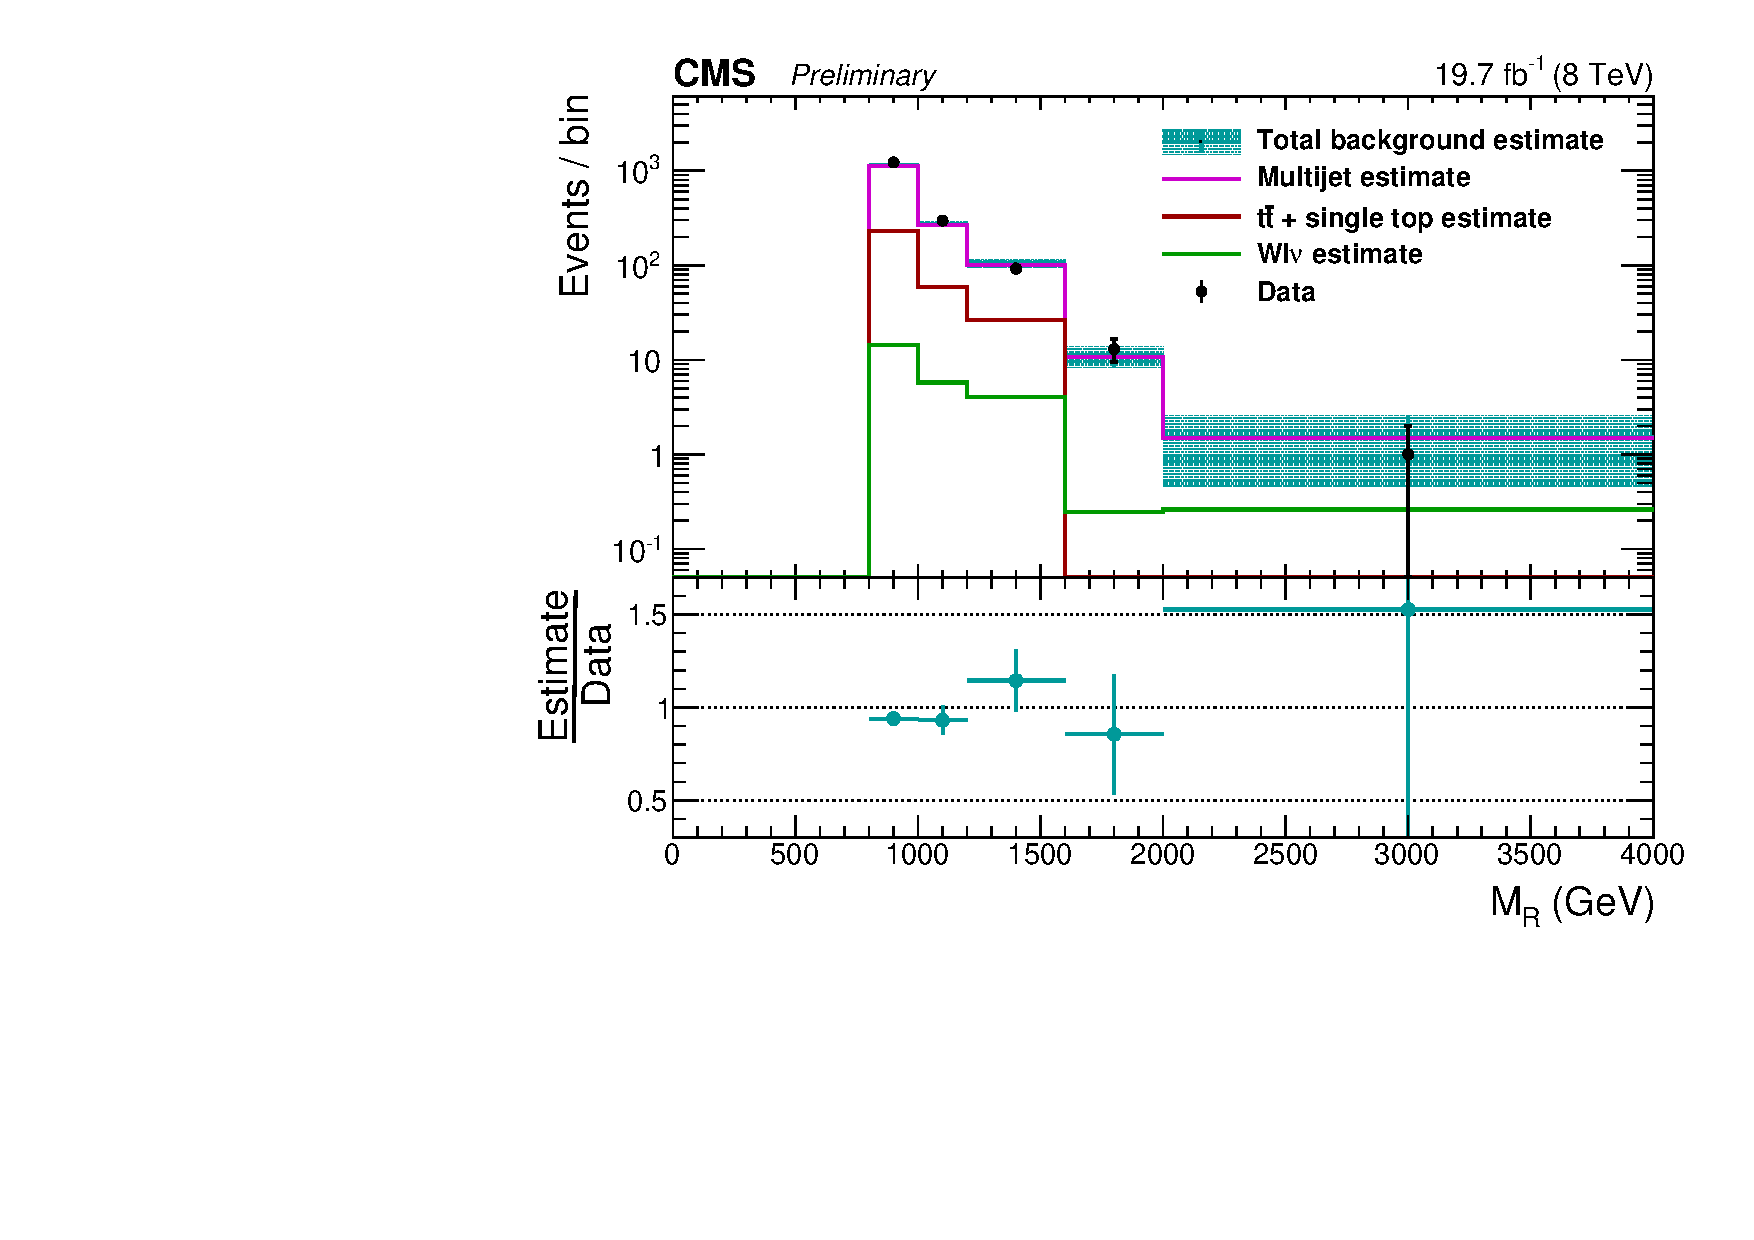
\includegraphics[width=0.48\textwidth]
{figures/razor_selection/MR_comparison_data_estimate_g1Mbg1W0Ll_mdPhi0p5_log}
~
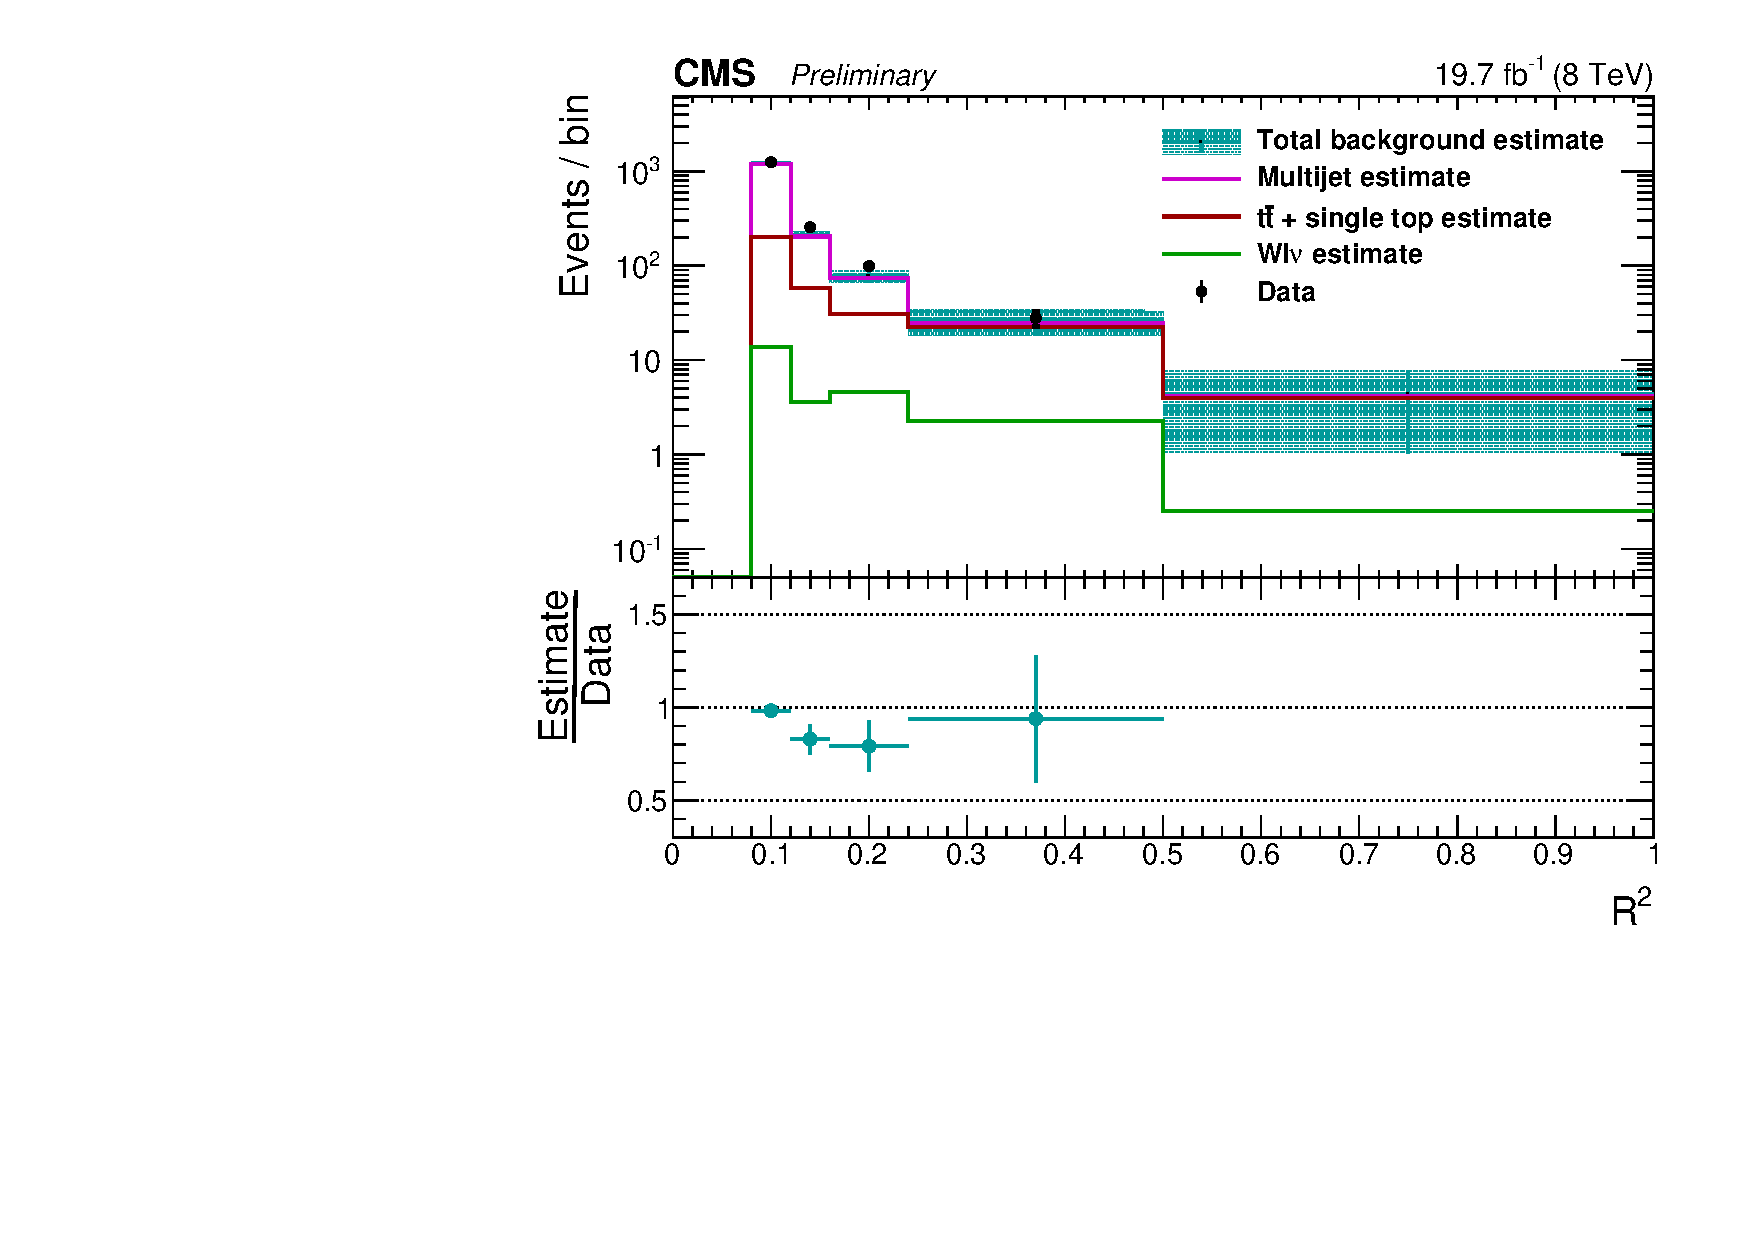
\includegraphics[width=0.48\textwidth]
{figures/razor_selection/R2_comparison_data_estimate_g1Mbg1W0Ll_mdPhi0p5_log}
\caption{Projection of the 2D prediction on the $\mr$ (left) and $\rsq$ (right) axes for the closure
test predicting the $\Delta\phi_{min}$ sideband region $S'$. The uncertainties shown are statistical
only and the horizontal error bars only indicate the bin width.
\label{fig:Shape_syst_1D_project_sideband}}
\end{figure}


\subsubsection{Second cross check}

In a second cross check, we use the $Q$ region to estimate the background in a more signal-like $Q$
region, denoted by $Q^\prime$, where $\Delta\phi_{min} > 0.5$. 
The selection is also summarized in Table~\ref{tab:boost_selection_summary}. 
The estimated background in the $Q'$ region, $\hat{N}^{Q^\prime}$, is computed as
\begin{equation}
  \hat{N}^{Q^\prime} = N_{\rm obs}^Q \frac{N_{\rm MC}^{Q^\prime}}{N_{\rm MC}^Q},
\end{equation}
where $N_{\rm obs}^Q$ is the observed data count in the $Q$ region, and
$N_{\rm MC}$ includes all contributing simulated background processes.

This test assesses the degree to which the simulated distribution of $\Delta\phi_{min}$ as well as
its extrapolation from the $Q$ region, which has $\Delta\phi_{min} < 0.3$, to the $S$ region, with
$\Delta\phi_{min} > 0.5$, are reliable. The comparison between
prediction and observation is shown in Fig.~\ref{fig:Shape_syst_1D_project_QCD}. 
The level of discrepancy, ${\sim}\,40\%$, between the prediction and observation in this cross
check is incorporated as a systematic uncertainty in the global scale factors. How this is done
technically is described in Section~\ref{sec:boost_likelihood}.

\begin{figure}[htpb]
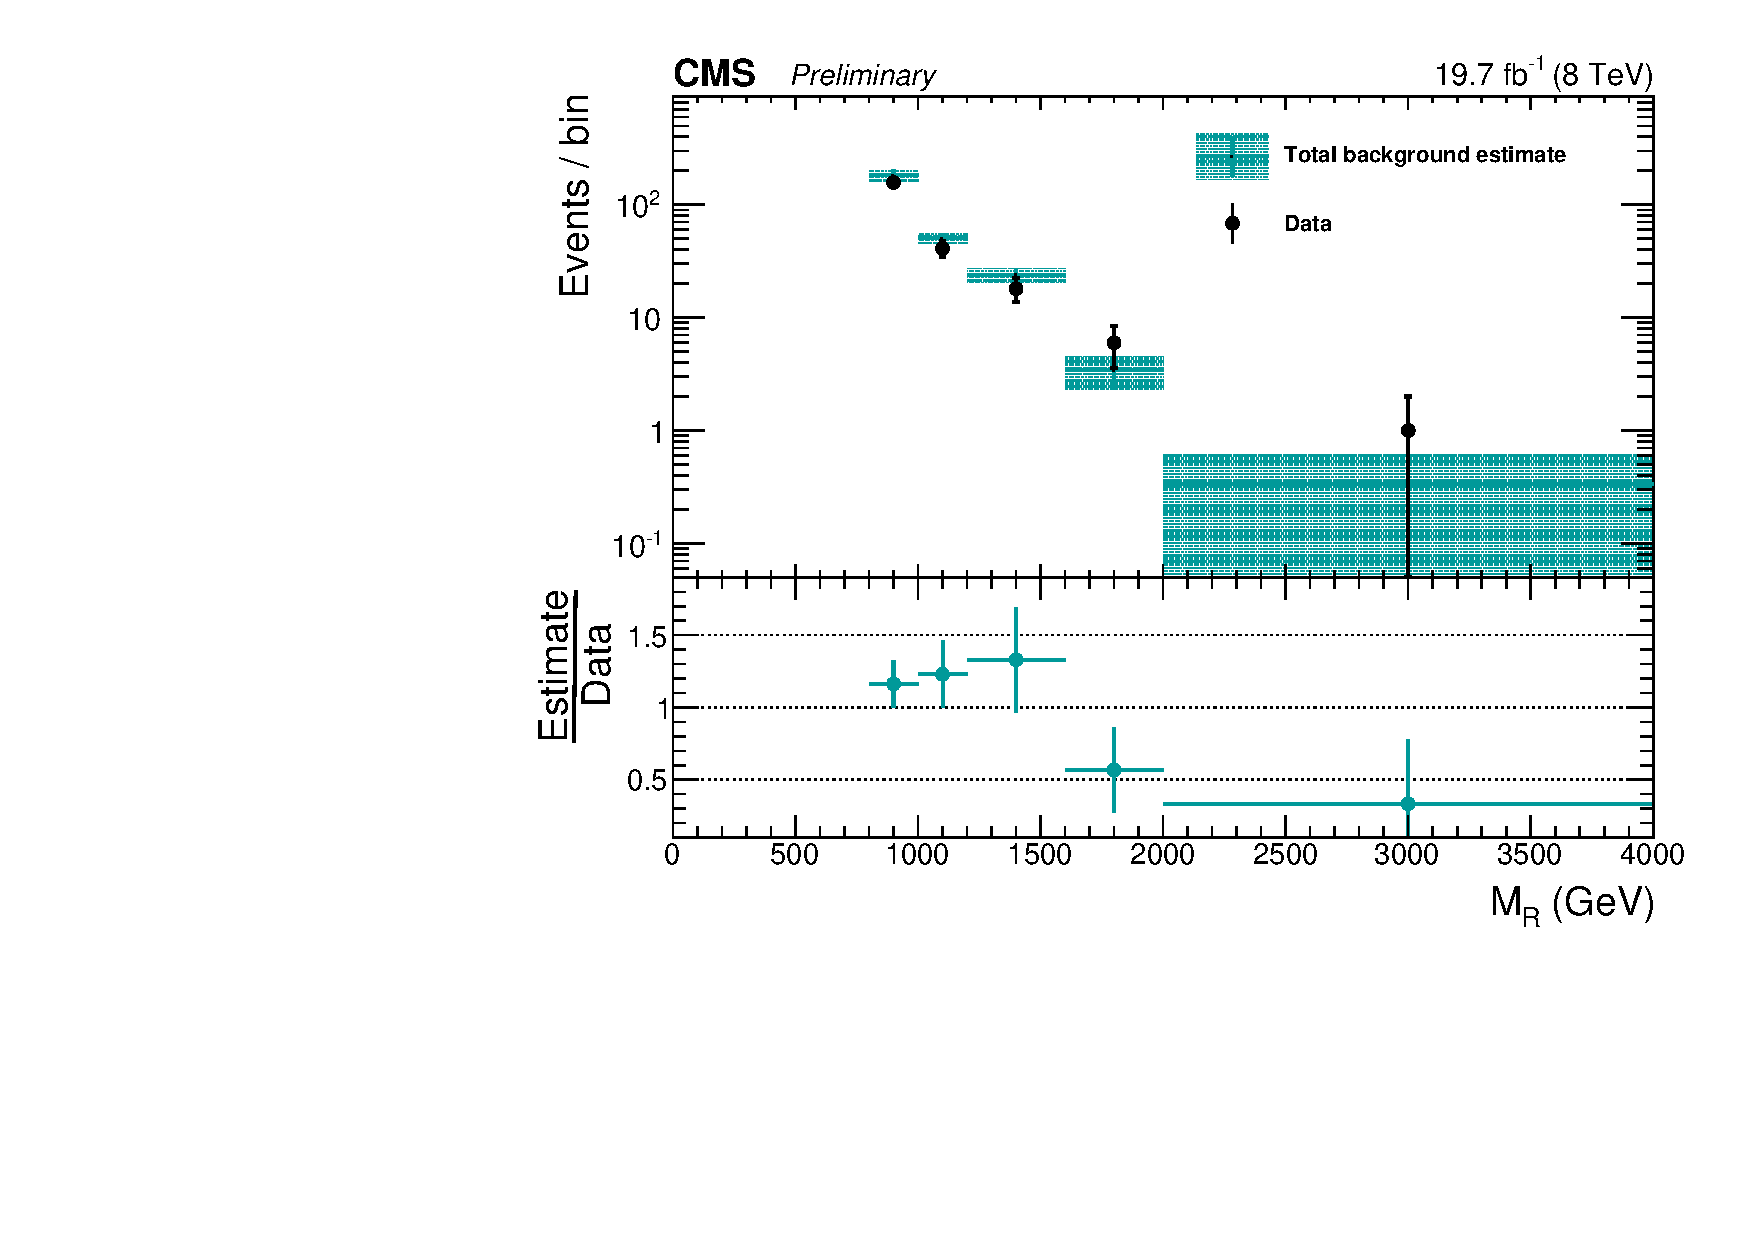
\includegraphics[width=0.5\textwidth]
{figures/razor_selection/MR_comparison_data_estimate_0Lbg1uW0Ll_mdPhig0p5_from_0Lbg1uW0Ll_mdPhi0p3_log}
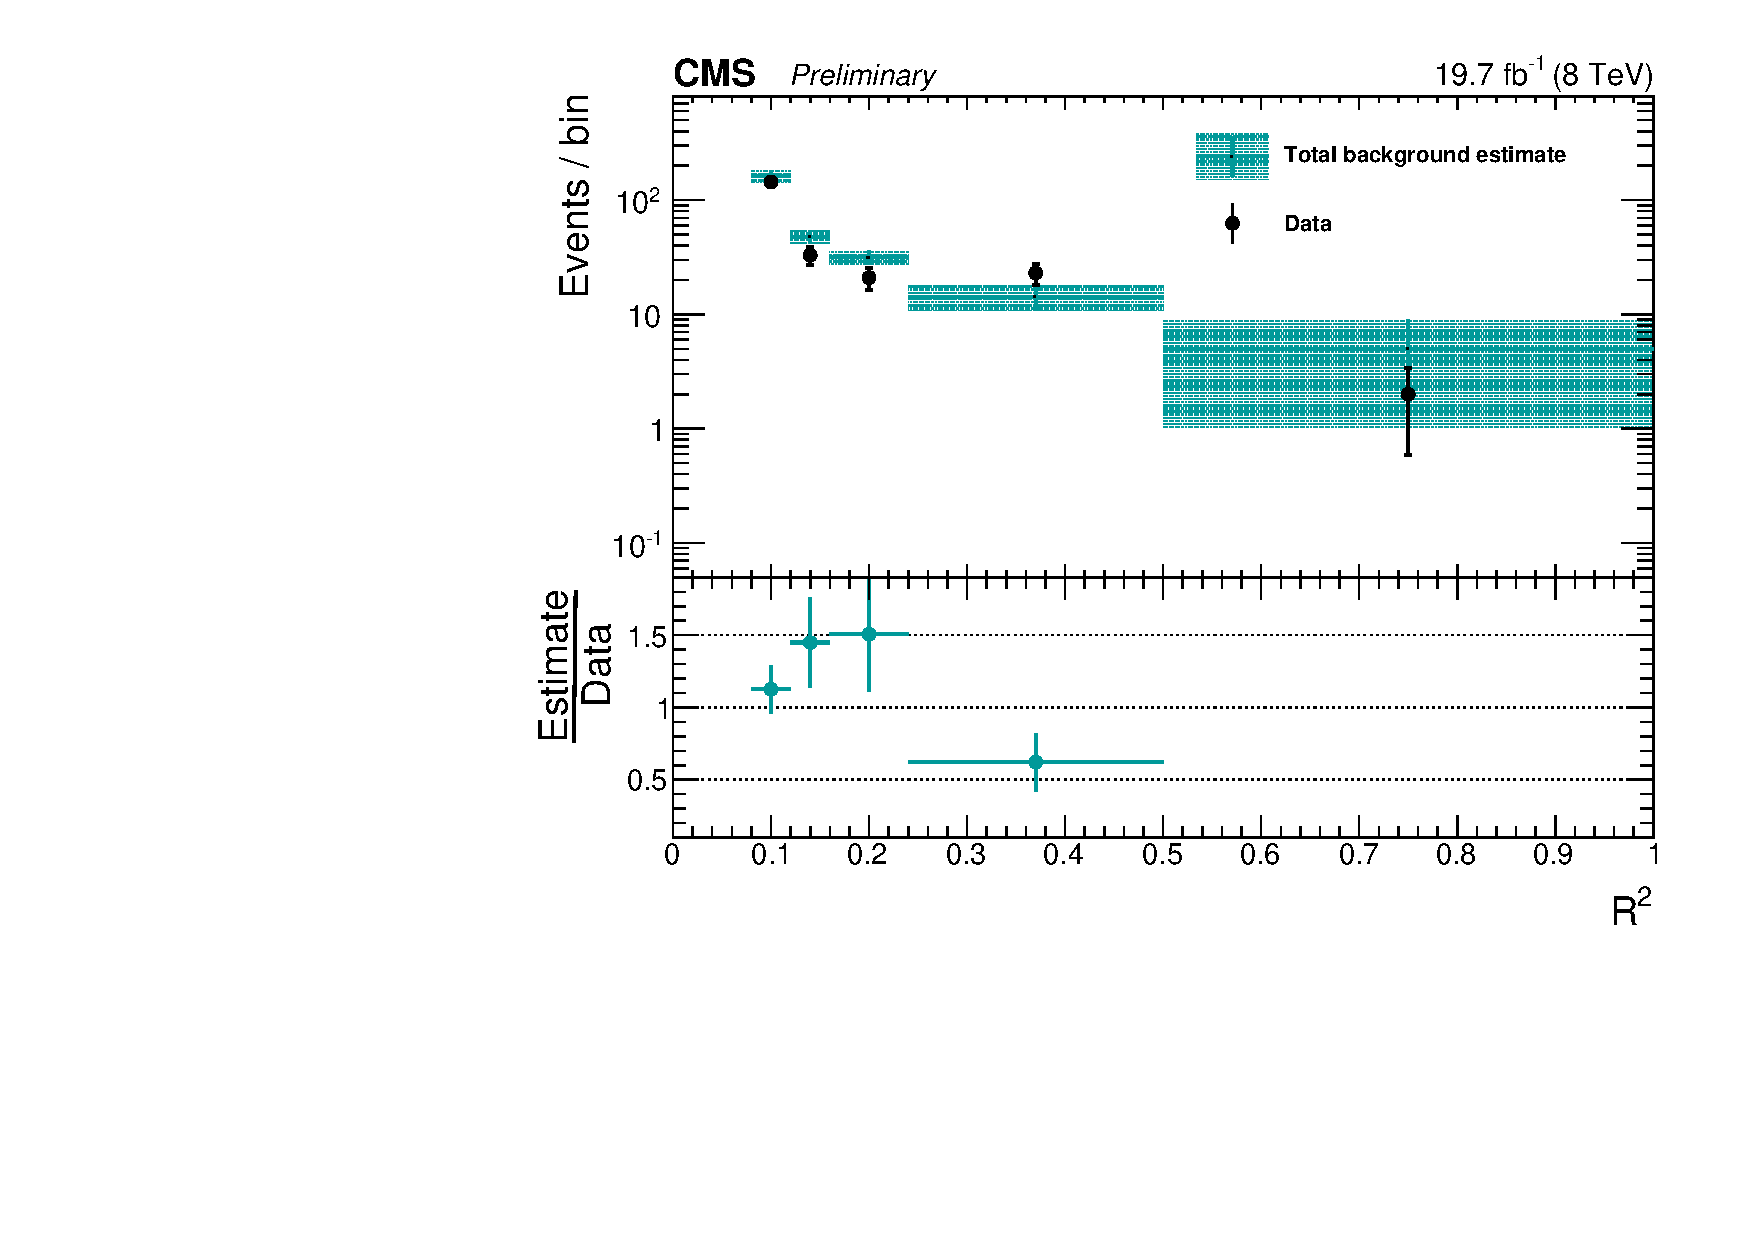
\includegraphics[width=0.5\textwidth]
{figures/razor_selection/R2_comparison_data_estimate_0Lbg1uW0Ll_mdPhig0p5_from_0Lbg1uW0Ll_mdPhi0p3_log}
\caption{Projection of the 2D prediction on the $\mr$ (left) and $\rsq$ (right) axes for the closure
test predicting the background in region $Q'$, as defined in the text. The uncertainties shown are
statistical only and the horizontal error bars only indicate the bin width.
\label{fig:Shape_syst_1D_project_QCD}}
\end{figure}
